\chapter{杠杆与天平}\label{ch:g3:levers-and-scales}

去年在跷跷板上，我们发现重力和距离都起作用，
--- 我们还许诺要给出一条含真实数字的精确规则。
现在就来兑现承诺。途中我们要举起重得手臂抬不动的石头，
还将认识一种为世界称量货物的仪器，
它为世界称量货物已有数千年。

\section{杠杆}

\begin{definition}[杠杆与支点]\label{def:g3:levers-and-scales:lever}
称\emph{杠杆}\index{杠杆}为一根硬棒，它搁在一个支撑点上，
并可以绕这个点转动。该支撑点称为
\emph{支点}\index{支点}。跷跷板是杠杆，压在石头下的撬棍也是，
拔钉子时的锤爪同样是杠杆。
\end{definition}

\begin{example}[力量放大器]\label{ex:g3:levers-and-scales:crowbar}
一位园丁把一根长铁棍塞到大石头底下，
让它搁在紧靠石头的圆木上，压住远端 --- 那块十个人都抬不动的石头
便被轻轻撬翻。杠杆的秘诀在于距离：
离支点越\emph{远}去用力，
小小一按，就抵得上靠近支点时的巨人之力。
一个古老的故事说，古代一位伟大的科学家曾夸口说：
“给我一个立足之地，再给我一根足够长的杠杆，我就能撬动地球。”
\end{example}

\begin{omfigure}
\begin{tikzpicture}[scale=0.85]
  \draw[thick] (0,0) -- (11,0);
  % fulcrum: flat base on the ground, apex up at (7.6,0.55)
  \draw[thick, fill=omExo, fill opacity=0.3]
    (7.15,0) -- (8.05,0) -- (7.6,0.55) -- cycle;
  % the bar: one straight line resting on the apex and tangent to the
  % rock (computed: through (7.6,0.55), touching the circle at (9.10,0.03))
  \draw[very thick] (1.74,2.57) -- (9.10,0.03);
  % the rock, sitting on the ground, its edge on the bar's tip
  \draw[thick, fill=omExo, fill opacity=0.4] (9.3,0.62) circle (0.62);
  \node[font=\small] at (9.3,0.62) {石头};
  \draw[-Stealth, very thick, omThm] (1.74,3.5) -- (1.74,2.75);
  \node[left, font=\small, omThm] at (1.5,3.15) {远端小力};
  \node[below, font=\small] at (7.6,-0.3) {支点靠近石头};
\end{tikzpicture}

{\small 撬棍：远离支点的一小股力，
能撬起靠近它的一块重石。}
\end{omfigure}

\begin{omfigure}
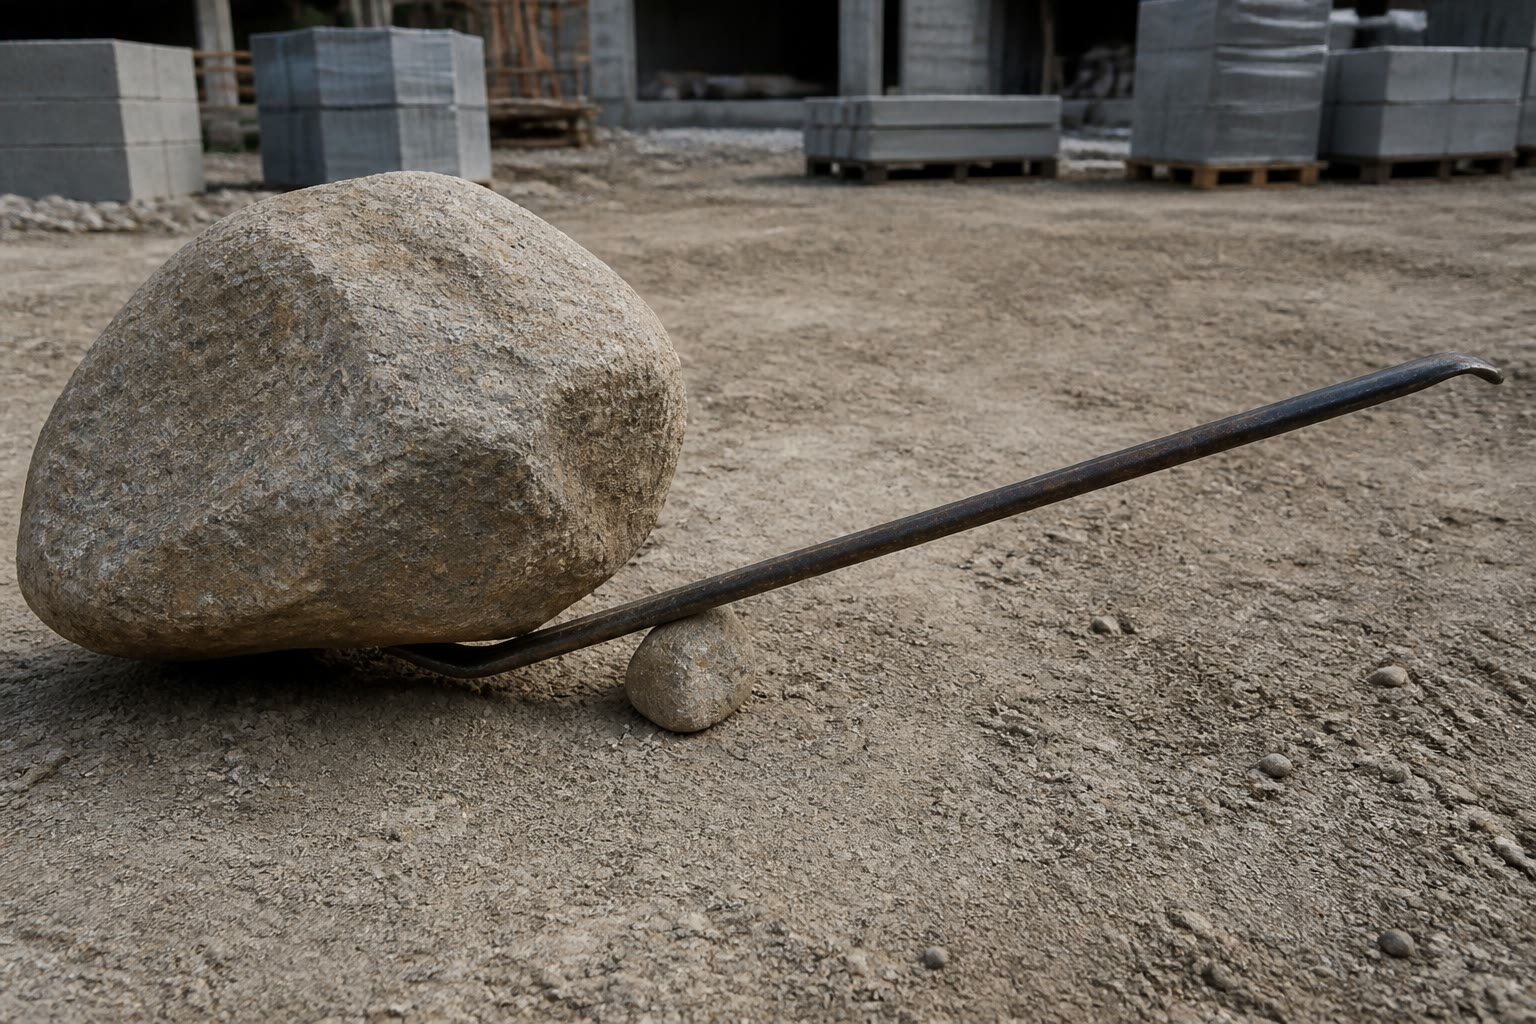
\includegraphics[width=0.55\linewidth]{images/book1/ai/g3-levers-crowbar.jpg}

{\small 撬棍工作时：远离支点的小力，能撬动一块人力都挪不动的巨石。}
\end{omfigure}

\section{杠杆法则}

\begin{method}[硬币跷跷板]\label{met:g3:levers-and-scales:coins}
搭一个迷你跷跷板，来探寻这条规律：
\begin{enumerate}
  \item 将尺子的中间刻度放在铅笔上，使尺子保持平衡；
  \item 用相同的硬币作为“骑手”，放在整数刻度上：
        “放在 $4$ 处的一枚硬币”指离铅笔四格；
  \item 两边都放上硬币，记下尺子何时平衡。
\end{enumerate}
试一试：$6$ 处的一枚硬币与另一侧 $6$ 处的一枚硬币平衡。两枚硬币叠放在
$3$ 处，可与 $6$ 处的一枚硬币平衡。三枚硬币放在 $2$ 处 --- 又与
$6$ 处的一枚硬币平衡！
\end{method}

\begin{proposition}[杠杆法则]\label{prop:g3:levers-and-scales:rule}
对杠杆的每一侧，把硬币个数乘以它们离支点的距离。
杠杆恰好平衡，当且仅当两侧
\emph{乘积相等}：
\[
2 \text{ 枚硬币} \times 3 \text{ 格} = 6
\qquad\text{平衡}\qquad
1 \text{ 枚硬币} \times 6 \text{ 格} = 6 .
\]
若一侧的乘积更大，那一侧就会下沉。
\end{proposition}

\begin{omfigure}
\begin{tikzpicture}[scale=0.85]
  \draw[thick, fill=omExo, fill opacity=0.3]
    (5.5,0) -- (5.9,0.7) -- (5.1,0.7) -- cycle;
  \draw[very thick] (1.0,0.78) -- (10.0,0.78);
  \foreach \x in {1.75,2.5,3.25,4.0,4.75,6.25,7.0,7.75,8.5,9.25} {
    \draw (\x,0.7) -- (\x,0.86);
  }
  \draw[thick, fill=omDef, fill opacity=0.5] (3.25,1.09) circle (0.3);
  \draw[thick, fill=omDef, fill opacity=0.5] (3.25,1.69) circle (0.3);
  \node[above, font=\small] at (3.25,2.1) {$2$ 枚硬币在 $3$ 处};
  \draw[thick, fill=omThm, fill opacity=0.5] (9.25,1.09) circle (0.3);
  \node[above, font=\small] at (9.25,1.5) {$1$ 枚硬币在 $6$ 处};
  \node[below, font=\small] at (5.5,-0.25)
    {左边 $2 \times 3 = 6$，右边 $1 \times 6 = 6$：
     平衡};
\end{tikzpicture}

{\small 尺子上的杠杆法则：乘积相等，横杆水平。}
\end{omfigure}

\begin{example}[法则的应用]\label{ex:g3:levers-and-scales:using}
四枚硬币放在 $2$ 处，乘积为 $4 \times 2 = 8$。要
用放在 $4$ 处的硬币与之平衡，那里的乘积也需为 $8$。
即 $8 = 2 \times 4$，所以放两枚硬币在 $4$ 处即可。那么一枚硬币
能否与这四枚平衡？它须放在 $8$ 处：$1 \times 8
= 8$。骑手越轻，就必须放得越远 --- 这正是
爸爸的跷跷板教给我们的道理，如今有了数字。
\end{example}

\section{天平}

\begin{definition}[天平]\label{def:g3:levers-and-scales:scale}
\emph{天平}\index{天平}是一种为公平而设计的杠杆，
两个托盘挂在离支点\emph{距离完全相等}的位置。
距离相等时，两边乘积恰好相等的条件是重量相等，
因此天平向较重的一侧倾斜，
两盘载重相等时则保持水平。
\end{definition}

\begin{omfigure}
\begin{tikzpicture}[scale=0.85]
  \draw[thick] (5.5,0) -- (5.5,2.6);
  \draw[thick] (4.9,0) -- (6.1,0);
  \draw[very thick] (2.5,2.6) -- (8.5,2.6);
  \fill (5.5,2.6) circle (2.4pt);
  \draw[thick] (2.5,2.6) -- (2.2,1.5) (2.5,2.6) -- (2.8,1.5);
  \draw[thick] (1.9,1.5) .. controls (2.5,1.05) .. (3.1,1.5);
  \draw[thick] (8.5,2.6) -- (8.2,1.5) (8.5,2.6) -- (8.8,1.5);
  \draw[thick] (7.9,1.5) .. controls (8.5,1.05) .. (9.1,1.5);
  \fill[omDef, opacity=0.5] (2.5,1.5) circle (0.28);
  \fill[omThm, opacity=0.5] (8.35,1.42) circle (0.22);
  \fill[omThm, opacity=0.5] (8.68,1.42) circle (0.22);
  \node[below, font=\small] at (5.5,-0.3)
    {等臂：天平公平地比较两个托盘};
\end{tikzpicture}

{\small 天平：两端托盘到支点距离相等的杠杆。
托盘水平即表示两边重量相等。}
\end{omfigure}

\begin{example}[通过比较称重]\label{ex:g3:levers-and-scales:weighing}
千百年来，商人们用天平售卖面粉、黄金和胡椒，
方法是一盘放货物，另一盘放小金属砝码，
不断增加砝码直到两盘水平。天平并不认识任何数字，
它只能回答“更重”“更轻”或“相等”。
但只要用选好的砝码进行比较，
公平的市场就已足够——正如本部分最后一章将说明的，
这正是测量质量本身的途径。
\end{example}

\begin{remark}[检查空载的天平]\label{rem:g3:levers-and-scales:fair}
公平的天平在\emph{空载}时必须保持水平。若一臂更长，
或一个托盘更重，那么在货物放上之前乘积就已不同，
此后每次称重都会作弊。诚实的商人
会当着顾客的面证明空载天平水平——这是一种古老的，
无需言语便能表达“公平交易”的做法。
\end{remark}

\section{练习}

\begin{exercise}[$\star$]\label{exo:g3:levers-and-scales:1}
指出下列物体中的杠杆和支点：跷跷板；\ 放在圆木上的撬棍；
\ 剪刀。（剪刀里藏着两个杠杆，它们的
支点在哪里？）
\end{exercise}

\begin{exercise}[$\star$]\label{exo:g3:levers-and-scales:2}
用撬棍撬起一块重石头时，应当靠近
支点用力，还是远离支点用力？请用一句话说明理由。
\end{exercise}

\begin{exercise}[$\star$]\label{exo:g3:levers-and-scales:3}
在硬币跷跷板上，计算下列情形的乘积：$3$ 枚硬币放在 $4$ 处；
\ $2$ 枚硬币放在 $5$ 处；\ $1$ 枚硬币放在 $6$ 处。哪些两组
可以互相平衡？
\end{exercise}

\begin{exercise}[$\star$]\label{exo:g3:levers-and-scales:4}
左侧 $8$ 处放一枚硬币。右侧应把 $2$ 枚硬币
放在哪里才能平衡？那 $4$ 枚呢？
\end{exercise}

\begin{exercise}[$\star$]\label{exo:g3:levers-and-scales:5}
左侧：$3$ 枚硬币放在 $3$ 处。右侧：$2$ 枚硬币放在 $4$ 处。
分别计算两侧的乘积。哪一侧会下沉？
\end{exercise}

\begin{exercise}[$\star$]\label{exo:g3:levers-and-scales:6}
为什么天平的两个托盘要挂在
距支点完全相等的位置？若左臂更长，每次称重
会受到什么影响？
\end{exercise}

\begin{exercise}[$\star$]\label{exo:g3:levers-and-scales:7}
天平水平时，一盘放一袋弹珠，另一盘放 $6$
块相同的砝码。由此能得出关于这袋弹珠的什么结论？
若拿走一块砝码，天平会给出什么结果？
\end{exercise}

\begin{exercise}[$\star$]\label{exo:g3:levers-and-scales:8}
一个跷跷板：汤姆的重量相当于 $2$ 袋，坐在 $3$ 处；他的
小妹妹的重量相当于 $1$ 袋，她应坐在哪里
才能与他平衡？
\end{exercise}

\begin{exercise}[$\star$]\label{exo:g3:levers-and-scales:9}
羊角锤拔钉子时，手按压锤柄的末端，
离锤头压在木头上的位置很远。哪一点是
支点？为什么连手指都拔不动的钉子，
用锤子却能拔出来？
\end{exercise}

\begin{exercise}[$\star\star$]\label{exo:g3:levers-and-scales:10}
爷爷（重量相当于 $4$ 袋）想和小佐伊（重量相当于
$1$ 袋）玩跷跷板。跷跷板两侧各有刻度 $1$ 至 $8$。请找出
\emph{两种}不同的就座方式，使跷跷板保持平衡。
\end{exercise}

\begin{exercise}[$\star\star$]\label{exo:g3:levers-and-scales:11}
一个奸诈的商人暗中把天平的一臂稍加长，
并总把货物放在长臂一侧。顾客拿到的货物是
比所付的多，还是少？请用杠杆
法则解释，并结合\cref{rem:g3:levers-and-scales:fair}作答。
\end{exercise}
